Pro návrh pásmové propusti 8. řádu s Cauerovou aproximací typu C byly zvoleny parametry tolerančního schématu $f_{-s} = 60$\,kHz, $f_{-p} = 150$\,kHz, $f_p = 190$\,kHz, $f_s = 280$\,kHz, $a_p = 1$\,dB a $a_s = 80$\,dB. 
Funkcí $BP2NLP$ byla provedena transformace tolerančního schematu nesymetrické pásmové propusti (PP) na toleranční schema normované dolní propusti (NDP). Byl spočítán nový kmitočet pro horní hranici nepropustného pásma $f_s = 101.786$\,kHz, geometrický střed propustného pásma $f_m = 168.819$\,kHz, šířka propustného pásma $\Delta{f_p} = 40$\,kHz a šířka nepropustného pásma $\Delta{f_s} = 178.314$\,kHz. Byl obdržen kmitočet hranice nepropustného pásma normované dolní propusti (NDP) $Os = 4.455$\,1/s.
\begin{figure}[h]
\centering
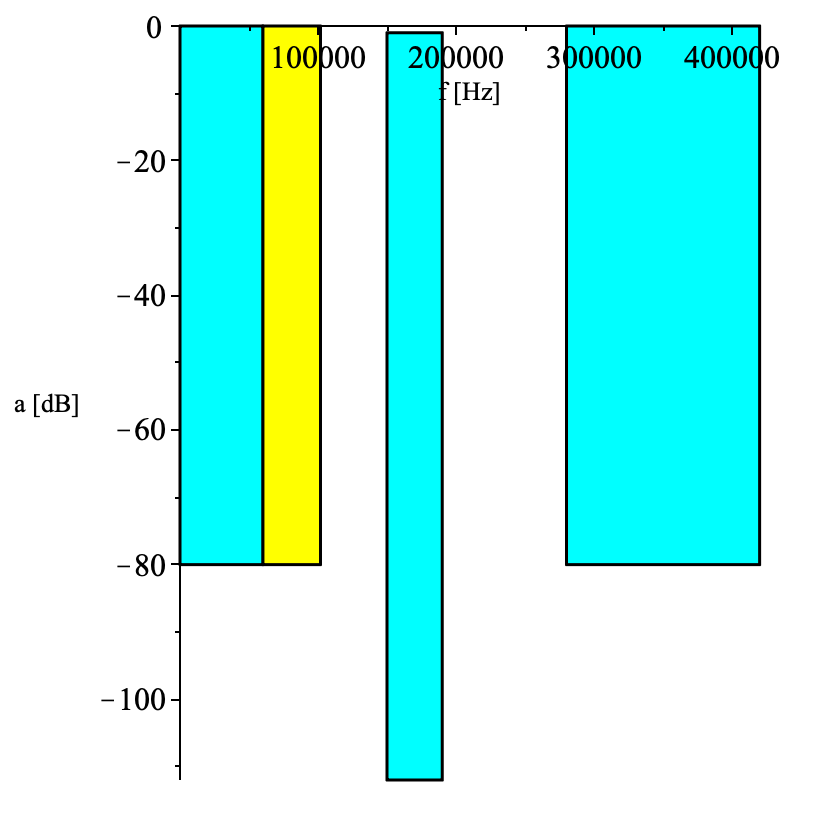
\includegraphics[scale=0.45]{tolsch2.png}
\caption{Toleranční schéma navrhované pásmové propusti}
\end{figure}
\noindent Stupeň Cauerovy aproximace normované dolní propusti byl určen jako $order = 4$. Pro Cauerovu aproximaci jsou definovány tři typy --- A, B, C. Tyto typy se od sebe liší průběhem aproximační funkce. Byla zvolena aproximace typu C se shodnými zakončovacími odpory.
\noindent Dále byla funkcí $Cauer\_asnew$ určena nová hodnota útlumu v~nepropustném pásmu NDP $a_{snew} = 81.719$\,dB.\\
\\
Následně byl spočten koeficient nejvyšší mocniny polynomu ve jmenovateli přenosové funkce $Gc = 94.811$, póly $P$ a nuly $Z$ přenosové funkce pomocí funkce $CauerCPolesZeros$. Počet pólů je dán řádem filtru $order$ a počet nul pro aproximaci typu C je roven $order = 2$. Dále byla spočtena Caurerova aproximace typu C~---~provozní činitel přenosu $G$ jako racionální lomená funkce $G(p) = 1/H(p)$, charakteristická funkce $chf$ jako $\Phi(p)$ s nulami a póly na imaginární ose. Charakteristická funkce má shodný jmenovatel s $G(p)$.
\newpage
\begin{equation}
P = 
\begin{bmatrix}
0.478 + 0.343 I & -0.478 - 0.343 I & -0.161 + 0.983 I & -0.161 - 0.983 I
\end{bmatrix}
\end{equation}
\begin{align}
Z &=
\begin{bmatrix}
5.706 I & -5.706 I
\end{bmatrix}\\
G &= \frac{94.881p^4+121.138p^3+156.142p^2+100.507p+32.556}{p^2+32.556}\\
chf &= \frac{(94.811p^2+78.754)p^2}{p^2+32.556}
\end{align}
\begin{figure}[h]
\centering
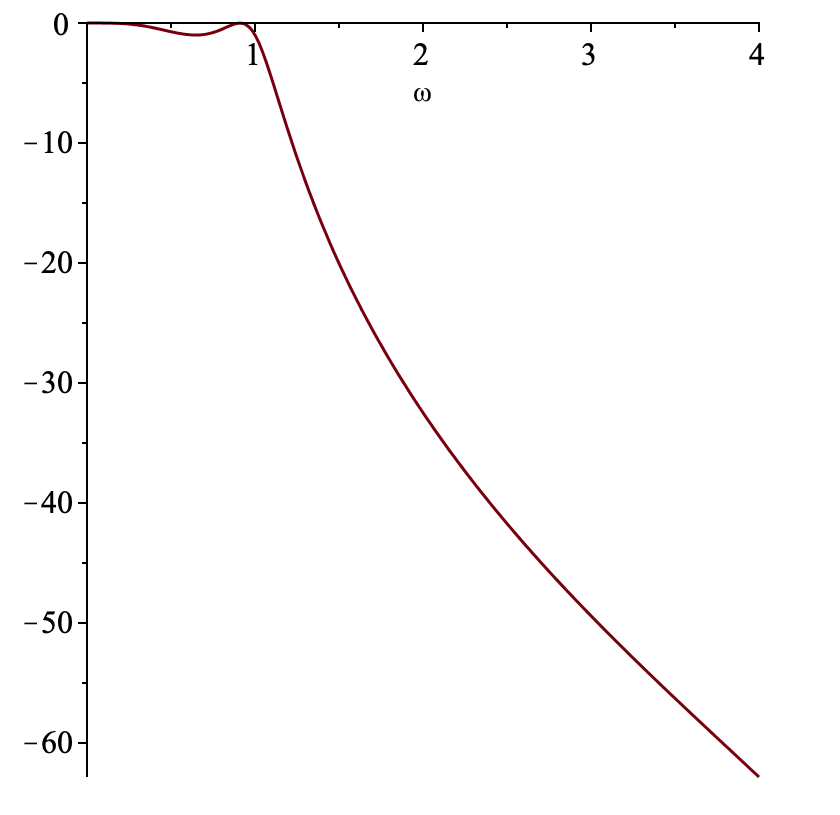
\includegraphics[scale=0.45]{sch02.png}
\caption{Modulová frekvenční charakteristika NDP}
\end{figure}
\subsection{Výpočet prvků LC filtru a přenosových funkcí}\label{s:VYP}
\noindent Funkcí $DroppNLP$ byly vypočteny prvky LC příčkového filtru typu normovaná dolní propust (NDP). Zakončení bylo zvoleno standardní (\textit{common}), odpory o hodnotě 1\,$\Omega$, směr zpracování od posledního prvku (\textit{rear}), s T strukturou. Standardní zakončení je oboustranné ($R_1~\neq~0, R_z~\neq~\infty$).
\MapleOutput{block (1), [orientation = direct, elements = {L1 = 1.571}, Z = p L1]}
\MapleOutput{block (2), [orientation = shunt, elements = {C1 = 1.542}, Z = \frac{1}{pC1}]}
\MapleOutput{block (3), [orientation = direct, elements = {C1 = 0.02, L1 = 1.522}, Z = \frac{1}{\frac{1}{pL1} + pC1}]}
\MapleOutput{block (4), [orientation = shunt, elements = {C1 = 1.545}, Z = \frac{1}{pC1}]}
\noindent Byl spočten  napěťový i~výkonový přenos.
\begin{align}
H_{NLPV} &= \frac{p^2  + 32.556}{190.352p^4  + 242.742p^3  + 312.889p^2  + 201.21p + 65.112}\\
H_{NLP} &= \frac{p^2  + 32.556}{95.176p^4 + 121.371p^3 + 156.444p^2 + 100.605p + 32.556}
\end{align}
\noindent Z rozložení pólů je patrné, že obě přenosové funkce jsou stabilní.
\begin{align}
190.352s_1^4 + 242.742s_1^3 + 312.889s_1^2 + 201.21s_1 + 65.112 &= 0 \\
95.176s_2^4 + 121.371s_2^3 + 156.444s_2^2 + 100.605s_2 + 32.556 &= 0
\end{align}
\begin{align}
s &= {-0.477 - 0.343 I}, {-0.477 + 0.343 I}, {-0.161 - 0.983 I}, {-0.161 + 0.983 I}
\end{align}
\begin{figure}[h]
\centering
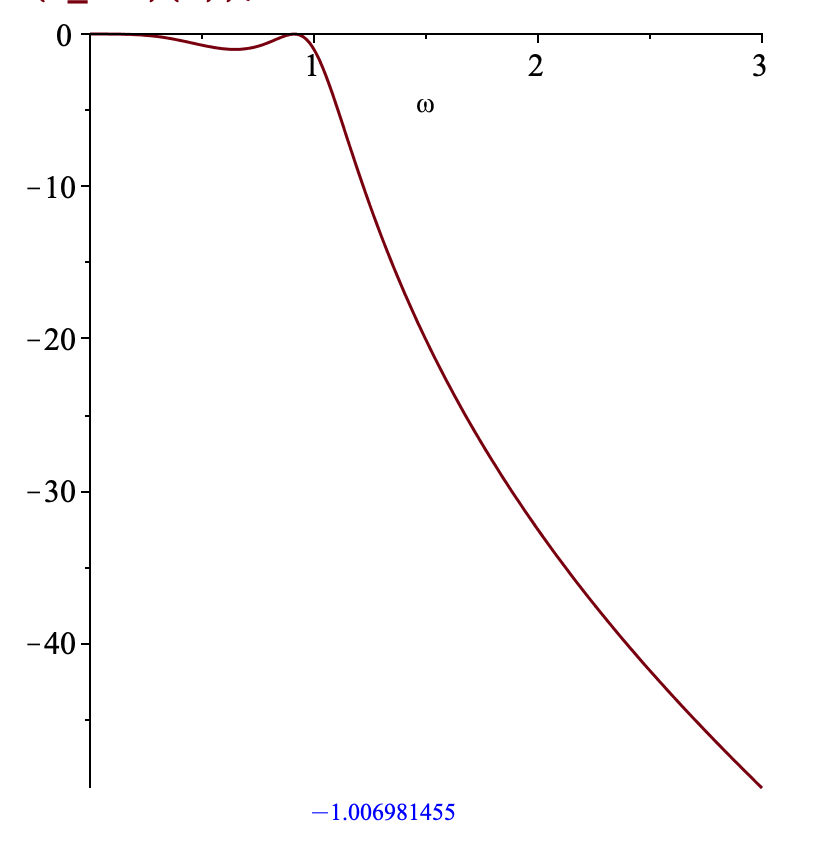
\includegraphics[scale=0.45]{sch022.png}
\caption{Modulová frekvenční charakteristika NDP - LC příčkový filtr}
\end{figure}
\noindent Hodnota přenosové funkce v 1 byla vyhodnocena jako $-1.007$.\\
\noindent Byla provedena transformace hodnot prvků normované dolní propusti (NDP) na~pásmovou propust (PP). Zakončovací rezistor byl zvolen 1\,$\Omega$.\\
Prvky v první větvi obvodu byly vyčísleny jako $C_1 = 1.422$e-7\,F, $L1 = 6.252$e-6\,H, v druhé větvi $C_2 = 6.135$e-6\,F, $L_2 = 1.449$e-7\,H. Pro třetí větev $C_3 = 8.031$e-8\,F, $C_4 = 1.468$e-7\,F, $L_3 = 1.107$e-5\,H, $L_4 = 6.055$e-6\,H a pro čtvrtou $C_5 = 6.149$e-6\,F, $L_5 = 1.445$e-7\,H.\\
\noindent Vygenerovaná struktura je popsána na obrázku \ref{s:SCHEM}.\\
\\
\begin{figure}[h]
\centering
\resizebox{12cm}{!}{
\figppp{Circuit(1)}{5.566}{2.075}{}{}}
\caption{Schéma LC příčkové struktury \label{s:SCHEM}}
\end{figure}
\noindent Byly nastaveny jakosti cívek v LC příčkové struktuře na konečnou hodnotu. Funkce $MakeRealL$ zařadí do výsledné LC příčkové struktury sériově rezistory k induktorům podle zadaného činitele jakosti $Q$ a zadaného kmitočtu.\\
\\
Pro první větev je $R_{s1} = 0.066$\,$\Omega$, pro druhou $R_{s2} = 0.002$\,$\Omega$, pro třetí $R_{s3} = 0.117$\,$\Omega$ a $R_{s4} = 0.064$\,$\Omega$.\\
\\
\noindent Byl spočten přenos pro LC strukturu bez a s přidanými sériovými rezistory. Pro oba přenosy byla vykreslena modulová frekvenční charakteristika. Přenosové funkce zde pro svou složitost a zachování přehlednosti textu nejsou uváděny, ale jsou k nalezení v přiloženém Maple skriptu.
\begin{figure}[h]
\centering
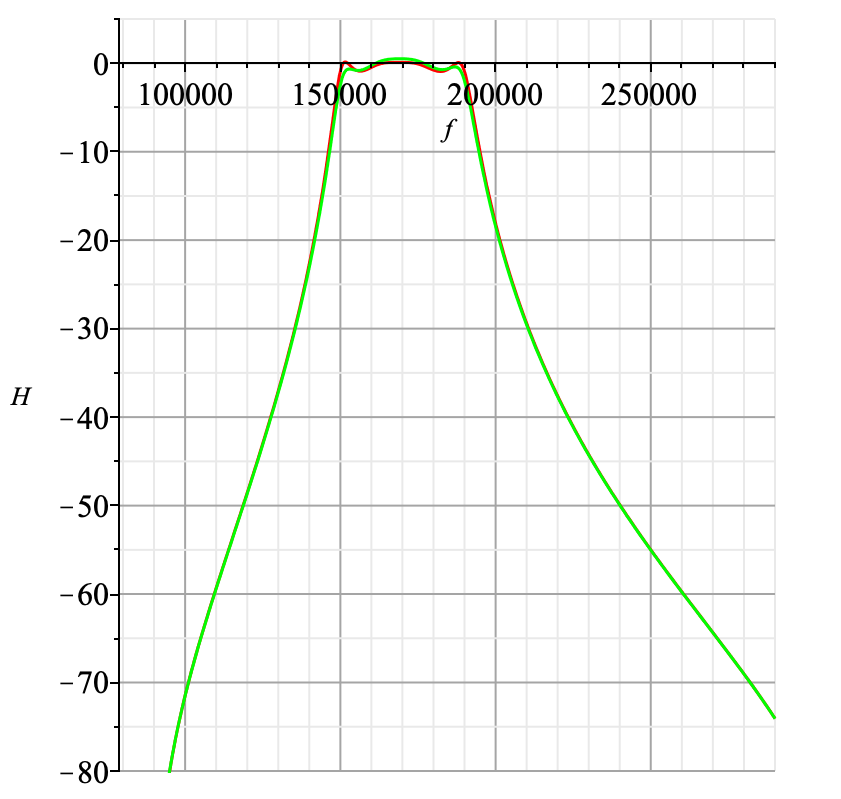
\includegraphics[scale=0.55]{modul12.png}
\caption[Modulová frekvenční charakteristika LC struktury a LC struktury s konečnou hodnotou jakostí cívek]{Modulová frekvenční charakteristika LC struktury (červená) a LC struktury s konečnou hodnotou jakostí cívek (zelená)}
\end{figure}
\begin{figure}[h]
\centering
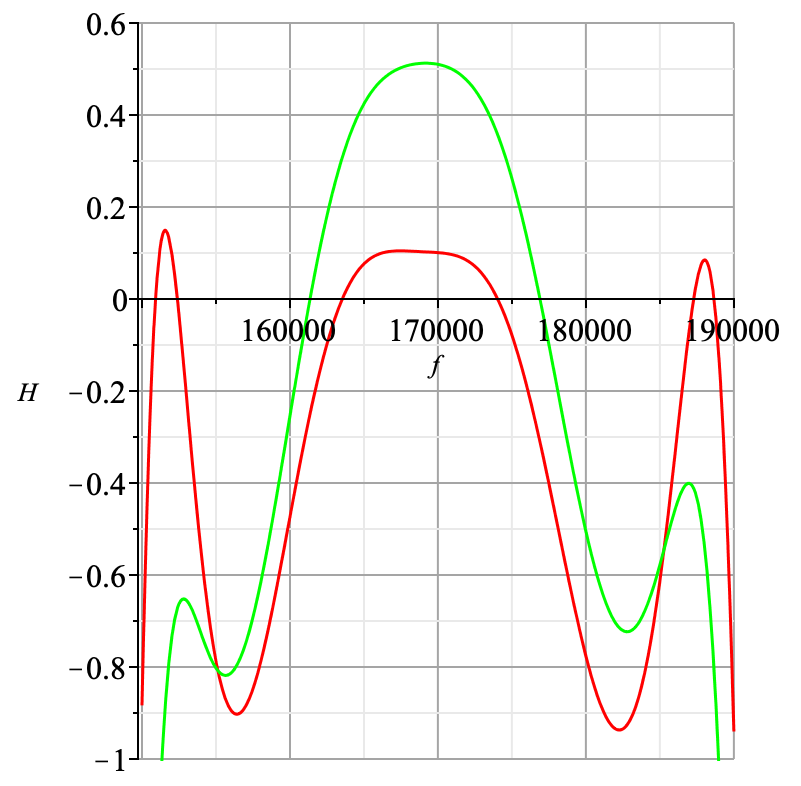
\includegraphics[scale=0.55]{modul123.png}
\caption[Přiblížená modulová frekvenční charakteristika LC struktury a LC struktury s konečnou hodnotou jakostí cívek]{Přiblížená modulová frekvenční charakteristika LC struktury (červená) a LC struktury s konečnou hodnotou jakostí cívek (zelená)}
\end{figure}
\noindent Vyčíslením v $f_m \cdot 2 \pi$ Hz, kde $f_m$ je geometrický střed propustného pásma, bylo obdrženo zesílení 0.283\,dB.\\
\\
\subsection{Simulace prvků LC prototypu}\label{s:ARC}
V této sekci byl náhradou induktorů v LC prototypu za gyrátory obdržen návrh ARC filtru.\\
Zatím neodnormované prvky byly vyčísleny jako $C_1 = 1.422$e-7\,F, $C_2 = 6.135$e-6\,F, $C_3 = 1.468$e-7\,F, $C_4 = 8.031$e-8\,F, $C_5 = 6.149$e-6\,F, $L_1 = 6.252$e-6\,H, $L_2 = 1.449$e-7\,H, $L_3 = 6.055$e-6\,H, $L_4 = 1.107$e-5\,H, $L_5 = 1.445$e-7\,H, $R_1 = 1$\,$\Omega$, $R_z = 1$\,$\Omega$.\\
\\
\noindent Odnormované hodnoty kapacit získané vydělením kmitočtem $fp \cdot 2 \pi$, kde $fp$ je horní hranice propustného pásma, byly spočteny jako $C_1 = 1.191$e-13\,F, $C_2 = 5.139$e-12\,F, $C_3 = 1.23$e-13\,F, $C_4 = 6.727$e-14\,F, $C_5 = 5.151$e-12\,F.\\
\noindent Frekvenčně a impedančně odnormované odpory byly vypočteny podělením kmitočtem $fp \cdot 2 \pi$ a přibližnou hodnotou kapacity pro mikroelektronickou realizaci $C = 2$\,pF. Výsledné hodnoty jsou $R_1 = R_z = 418.828$\,k$\Omega$.\\
\noindent Využitím poznatků ze sekce \ref{s:GYR} byly dosazením do vztahu $C = L \cdot g_m^2$ s uvažováním minimální transkonduktance z datasheetu LM13700 ($g_m$ = 9600\,$\upmu$S) získány kapacity $C_{L1} = 5.762$e-10\,F, $C_{L2} = 1.335$e-11\,F, $C_{L3} = 5.58$e-10\,F, $C_{L4} = 1.02$e-15\,F, $C_{L5} = 1.332$e-11\,F.\\
\\
\noindent Výsledné hodnoty všech součástek s přesností na dvě desetinná místa jsou\\ $C1 = 11.91$\,pF, $C2 = 5.14$\,pF, $C3 = 12.3$\,pF, $C4 = 672.74$\,pF, $C5 = 5.15$\,pF, $C_{L1} = 57.62$\,nF, $C_{L2} = 133.52$\,nF, $C_{L3} = 55.8$\,nF, $C_{L4} = 1019.9$\,pF, $C_{L5} = 133.21$\,nF, $R1 = Rz = 418.83$\,k$\Omega$.
\subsection{Funkční simulace LC prototypu}\label{s:KASK}
\noindent Analýzou LC struktury z Maplu byly obdrženy obvodové rovnice, kde R je volitelný (fiktivní) rezistor.
\begin{align}
I_1 &= \frac{1}{R_1 + pL_1 + \frac{1}{pC_1}}(U_G - U_2)\\
v_1 & = \frac{R}{R_1 + pL_1 + \frac{1}{pC_1}}(U_G - U_2)\\
U_2 &= \frac{1}{\frac{1}{pL_2} + pC_2}(I_1 - I_{3} - I_{L4} - pC_4 v_{L4})\\
U_2 &= \frac{1}{\frac{R}{pL_2} + RpC_2}(v_1 - v_{L3} - v_{L4} - RpC_4 U_{L4})\\
I_{3} &= \frac{1}{pL_3 + \frac{1}{pC_3}}(U_2 - U_3)\\
v_{L3} &= \frac{R}{pL_3 + \frac{1}{pC_3}}(U_2 - U_3)\\
v_{L4} &= \frac{1}{\frac{1}{pL_4}+pC_4}(I_1 - I_{L2} - pC_2U_2 - I_{3} - pC_4 (U_2 - U_3))\\
v_{L4} &= \frac{1}{\frac{R}{pL_4}+RpC_4}(v_1 - v_{L2} - RpC_2U_2 - v_{L3} - RpC_4 (U_2 - U_3))\\
U_3 &= \frac{1}{\frac{1}{R_z}+pC_5 + \frac{1}{pL_5}}(I_1 - I_{L2} - pC_2U_2)\\
U_3 &= \frac{1}{\frac{R}{R_z}+RpC_5 + \frac{R}{pL_5}}(v_1 - U_2 - RpC_2 U_2)
\end{align}
\noindent To odpovídá realizační struktuře s pěti bloky o přenosech $H_1, \ldots,H_5$.
\begin{align}
H_1 & = \frac{R}{R_1 + pL_1 + \frac{1}{pC_1}}\\
H_2 &= \frac{1}{\frac{R}{pL_2} + RpC_2}\\
H_3 &= \frac{R}{pL_3 + \frac{1}{pC_3}}\\
H_4 &= \frac{1}{\frac{R}{pL_4}+RpC_4}\\
H_5 &= \frac{1}{\frac{R}{R_z}+RpC_5 + \frac{R}{pL_5}}
\end{align}
\noindent Tato struktura je příliš složitá na realizaci blokovou strukturou, proto s ní dále nebylo počítáno. 
\subsection{Simulace obvodu}
\noindent  Zapojení s OTA vychází z již uvedených principů v sekci \ref{s:NAH}. K simulaci byly použity vypočtené hodnoty ze sekce \ref{s:ARC}. \\
\\
Šířka propustného pásma byla pro klidový stejnosměrný pracovní proud $I_{ABC} = 50$\,$\upmu$A odečtena jako 110.75\,kHz (amplitudová a fázová charakteristika je na obrázku \ref{s:OTAPP} a \ref{s:OTAPP1}). Geometrický střed propustného pásma odpovídá 100\,kHz. Přeladěním filtru změnou klidového stejnosměrného pracovního proudu na $I_{ABC} = 100$\,$\upmu$A byla obdržena šířka propustného pásma 225.88\,kHz a geometrický střed propustného pásma 200\,kHz (viz obrázek \ref{s:OTAPP2} a \ref{s:OTAPP22}). \\
\\
Pro obdržení geometrického středu propustného pásma $f_m = 168.819$\,kHz je třeba zvolit klidový stejnosměrný pracovní proud $I_{ABC} = 84.4$\,$\upmu$A. Byla odečtena šířka propustného pásma 202.78\,kHz a útlum v propustném pásmu 6-9\,dB (viz obrázek \ref{s:OTAPP3} a \ref{s:OTAPP33}). \\
\\
Analýzou obvodu se zapojením PP 4. řádu (kaskádní zapojení obvodu z obrázku \ref{s:V1}) a obvodu s hodnotami komponent z Maplu bylo obdrženo bylo určeno THD a šum. Byl použit klidový stejnosměrný pracovní proud $I_{ABC} = 50$\,$\upmu$A odpovídající geometrickému středu propustného pásma 100~kHz. Šum zde byl počítán jako výkon signálu ve zvoleném uzlu vydělený celkovým výkonem tepelného šumu na standardní teplotě (27\,$^{\circ}$C). Jak lze vidět z tabulek \ref{s:THD1} a \ref{s:THD2}, odstup signál šum je nejmenší pro frekvenci 100\,kHz odpovídající geometrickému středu propustného pásma.
\begin{table}[h]
\centering
  \begin{tabular}{ | c | c | c |}
    \hline
     Frekvence [kHz] & Odečtený šum [dB] \\ \hline
    1 & 89.571 \\ \hline
    10 & 49.313 \\ \hline
    100 & 9.514 \\ \hline
    1000 & 45.341 \\ \hline
  \end{tabular}
  \caption[Šum pro PP 4. řádu (Maple)]{Šum pro PP 4. řádu s výsledky z Maplu \label{s:THD1}}
\end{table}
  \begin{table}[h]
\centering
  \begin{tabular}{ | c | c | c |}
    \hline
     Frekvence [kHz] & Odečtený šum [dB] \\ \hline
    1 & 145.616 \\ \hline
    10 & 68.576 \\ \hline
    100 & 21.531 \\ \hline
    1000 & 108.632 \\ \hline
  \end{tabular}
\caption[Šum pro PP 4. řádu]{Šum pro PP 4. řádu \label{s:THD2}}
\end{table}
\noindent Také bylo změřeno THD se základní frekvenci 100\,kHz, viz tabulka \ref{s:THD3} a \ref{s:THD4}. Dle očekávání je nejnižší pro nejmenší počet harmonických frekvencí.
\begin{table}[h]
\centering
\renewcommand{\arraystretch}{1.15}
  \begin{tabular}{ | c | c | c |}
    \hline
    Frekvence zdroje [kHz] & Počet harmonických frekvencí & THD [\%] \\ \hline
	\multirow{3}{*}{100} & 3 & 2.969\\& 5 & 3.102 \\& 10 & 3.125 \\ \hline
  \end{tabular}
  \caption[THD pro PP 4. řádu (Maple)]{THD pro PP 4. řádu s výsledky z Maplu \label{s:THD3}}
\end{table}
\begin{table}[h]
\centering
\renewcommand{\arraystretch}{1.15}
  \begin{tabular}{ | c | c | c |} 
    \hline
     Frekvence zdroje [kHz] & Počet harmonických frekvencí & THD [\%] \\ \hline
	\multirow{3}{*}{100} & 3 & 0.114\\& 5 & 0.216 \\& 10 & 0.267 \\ \hline
  \end{tabular}
  \caption[THD pro PP 4. řádu]{THD pro PP 4. řádu \label{s:THD4}}
\end{table}